\chapter{Experimenteller Aufbau und Messprinzip}

\begin{figure}[H]
    \centering
    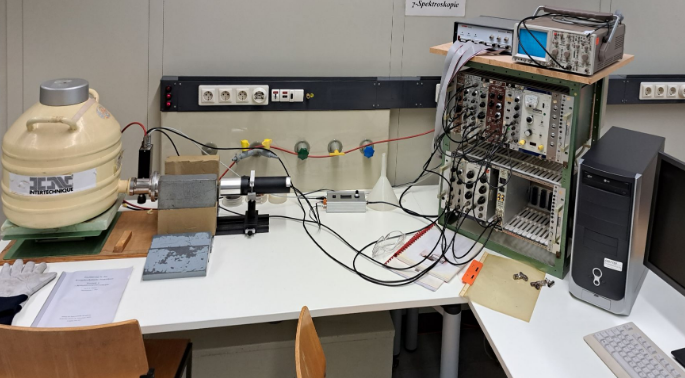
\includegraphics[width=0.7\linewidth]{include/Aufbau.png}
    \caption{Aufbau des $\gamma$-Spektroskopieexperiments. Links befindet sich der Ge-Detektor mit Vakuumflasche und NaJ-Detektor, rechts davon ist die Elektronik zur Datenaufnahme, sowie der Computer zur Analyse der Daten.}
    \label{fig:Aufbau}
\end{figure}

Die Detektoren erfassen $\gamma$-Strahlung und liefern jeweils zwei Signale: ein Energiesignal und ein Zeitsignal.

Die Energiesignale werden verstärkt und separat von ADC 1 (für den NaJ-Detektor) und ADC 2 (für den Ge-Detektor) digitalisiert. Sie liefern die Energieinformationen der registrierten Photonen.

Die Zeitsignale aus beiden Detektoren werden über schnelle Verstärker und sogenannte Constant Fraction Discriminators (CFDs) verarbeitet und zum TAC (Time-to-Analog Converter) geführt. Dieser misst die Zeitdifferenz zwischen den beiden Signalen, wobei der NaJ-Detektor das Startsignal und der Ge-Detektor – verzögert – das Stoppsignal liefert.

Der Ausgang des TAC ist ein analoges Spannungssignal, das der gemessenen Zeitdifferenz entspricht. Dieses Signal wird durch den dritten ADC (ADC 3) digitalisiert. Der dritte ADC ist daher zentral für die Koinzidenzmessung, da nur durch ihn die zeitliche Korrelation zwischen den beiden Ereignissen erfasst werden kann.

Durch die Kombination aller drei ADC-Werte (Energie 1, Energie 2, Zeitdifferenz) lassen sich echte Koinzidenzen identifizieren – also solche Ereignisse, bei denen zwei $\gamma$-Quanten innerhalb eines sehr kurzen Zeitfensters aus demselben Zerfall stammen. Damit bildet der dritte ADC die Grundlage für die spätere softwaregestützte Unterscheidung zwischen echten und zufälligen Koinzidenzen sowie für die Analyse von $\gamma$-Kaskaden.

\begin{figure}
    \centering
    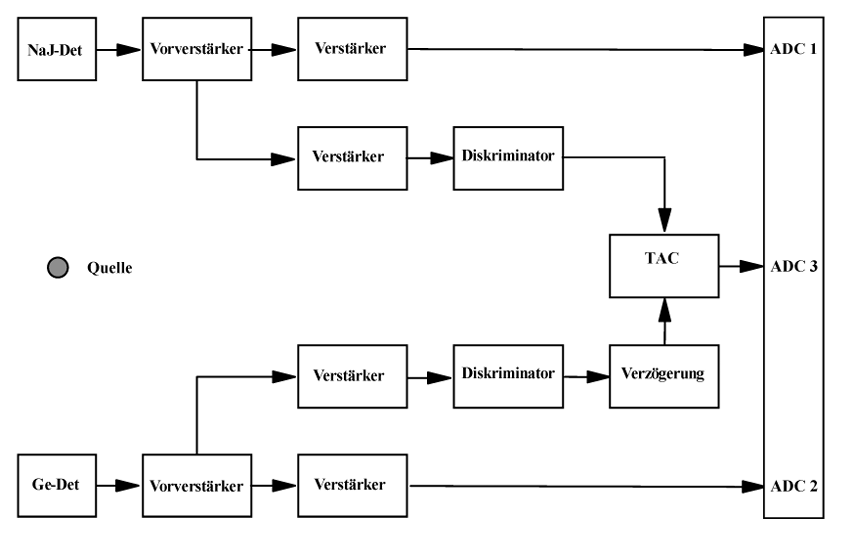
\includegraphics[width=0.5\linewidth]{include/Schaltplan.png}
    \caption{Blockschaltbild der Signalverarbeitungselektronik}
    \label{fig:Blockschaltbild}
\end{figure}